\subsubsection{Proceso: Consultar partidas}

\begin{itemize}
	\item \textbf{O1.1:} Busca todas las partidas dado el nombre del juego.
\end{itemize}

Esquema de navegabilidad: Ver figura \ref{fig:O1.1}.

\begin{figure}[h!]
	\centering
	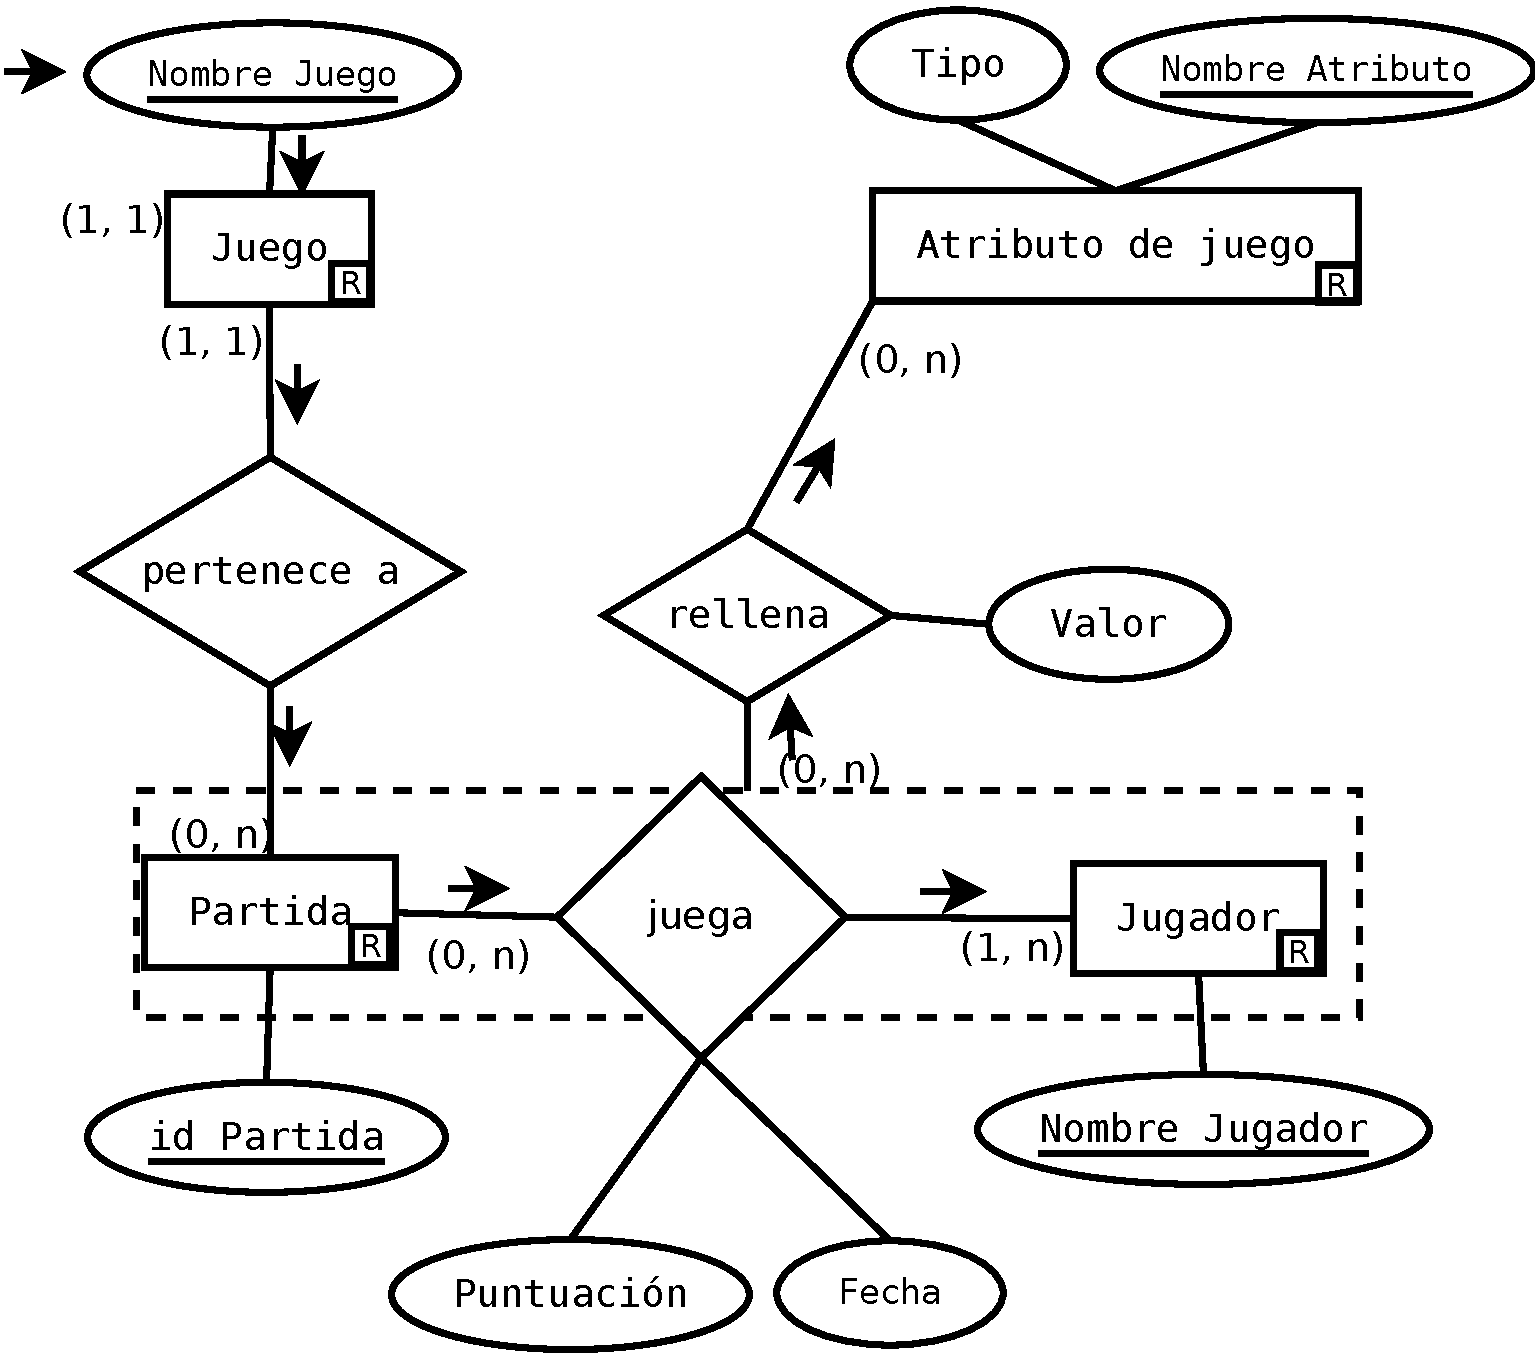
\includegraphics[width=0.7\linewidth]{../Diagramas/pdf/Op1-Consulta.pdf}
	\caption{Esquema de navegabilidad de la operación O1.1.}
	
	\label{fig:O1.1}
\end{figure}


\subsubsection{Proceso: Restricción de atributo}

\begin{itemize}
	\item \textbf{O1.2:} Busca las partidas (dado el nombre del juego) donde un atributo cumpla una condición dado por un valor.
\end{itemize}

Esquema de navegabilidad: Ver figura \ref{fig:O1.2}.

\begin{figure}[h!]
	\centering
	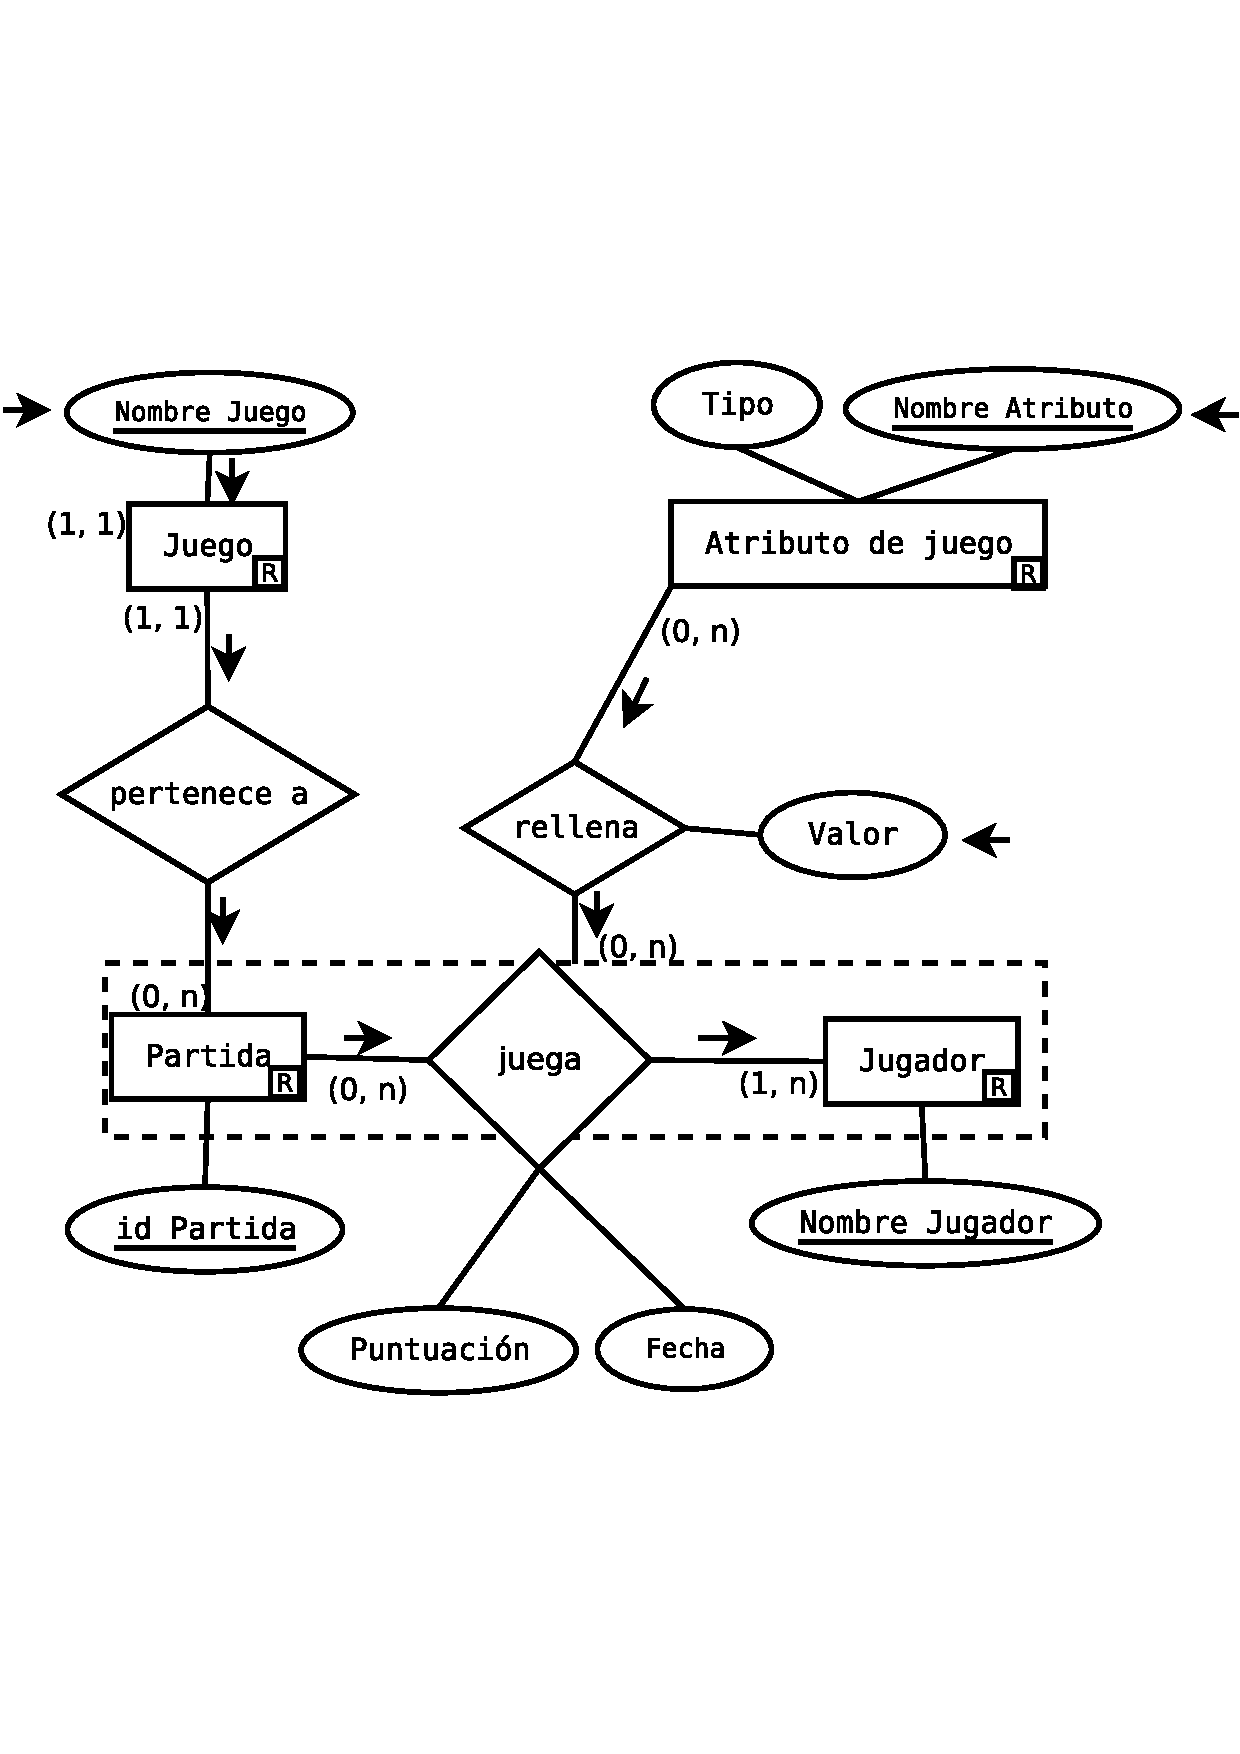
\includegraphics[width=0.7\linewidth]{../Diagramas/pdf/Op2-Consulta.pdf}
	\caption{Esquema de navegabilidad de la operación O1.2, O1.3 y O1.4.}
	
	\label{fig:O1.2}
\end{figure}


\subsubsection{Proceso: Unión de restricciones}

\begin{itemize}
	\item \textbf{O1.3:} Busca las partidas (dado el nombre del juego) donde un atributo cumpla una condición dado por varios valores, y devuelve las partidas que cumple alguna de estas condiciones.
\end{itemize}

Esquema de navegabilidad: Ver figura \ref{fig:O1.2}.

\textbf{Especificación}: Cada atributo tiene un valor dependiendo de la propia partida, y para \textbf{O1.3} se fijan varios atributos con un valor por cada atributo, para devolver las partidas que cumplan alguna de las condiciones.


\subsubsection{Proceso: Intersección de restricciones}

\begin{itemize}
	\item \textbf{O1.4:} Busca las partidas (dado el nombre del juego) donde un atributo cumpla una condición dado por varios valores, y devuelve las partidas que cumplen todas estas condiciones.
\end{itemize}

Esquema de navegabilidad: ver figura \ref{fig:O1.2}.

\textbf{Especificación}: Cada atributo tiene un valor dependiendo de la propia partida, y para \textbf{O1.4} se fijan varios atributos con un valor por cada atributo, para devolver las partidas que cumplan todas de las condiciones.
